\section{Durchführung}
\label{sec:Durchführung}
    \subsection{Bestimmung von D}
    Die Winkelrichtgröße D wird mit der Formel \ref{eqn:D} berechnet.
    Um diese Größen zu messen wird erst eine Eisenstange, die senkrecht zu Drehachse ausgerichtet ist, in der Halterung für die Körper befestigt.
    Nun wird eine Federwage in der Entfernung $r = 20$\unit{\centi\meter} von der Drehachse eingehängt.
    Dann wird diese um den Winkel $\varphi$ ausgelenkt und die Kraft wird an der Federwage abgelesen.
    Dabei muss die Federwage senkrecht zur Eisenstange sein, da dadurch der Sinus im Kreuzprodukt zu 1 wird und sich damit die Formel zu \ref{eqn:D2} vereinfacht.
    Die Messung wurde 11 mal durchgeführt und das arithmetische Mittel bestimmt um einen genaueren Wert zu erhalten.

    \subsection{Bestimmung von $I_D$}
    Um das Eigenträgheitsmoment $I_D$ zu bestimmen werden nun Gewichte an der Eisenstange angebracht. 
    Diese wird daraufhin um den Winkel $\varphi = 90$\unit{\degree}ausgelenkt und zum schwingen gebracht.
    Jetzt wird $5 \cdot T$ mit der Stoppuhr gemessen. 
    Der Faktor 5 wird verwendet um das Messen zu vereinfachen. 
    Diese Messung wird 10 mal für verschiedene Abstände a durchgeführt.
    %Das Eigenträgheitsmoment der Drillachse wird nun nach auftragen von $T^2$ zu $a^2$ durch lineare Regression bestimmt.%der Drillachse?

    \subsection{Bestimmung von $I$ verschiedener Körper}
    Die beiden Körper werden an der Halterung befestigt und um einen Winkel von $\varphi= 90$\unit{\degree} ausgelenkt.
    Mit der Stoppuhr wird $5 \cdot T$ bestimmt. 
    Dies wird 10 mal durchgeführt.% und das arithmetische Mittel bestimmt.
    %Da T nun bekannt ist kann mithilfe der Formel (Referenz aus dem Theorieteil einfügen) ${I}$ ausgerechnet werden.

    \subsection{Bestmmung von $I$ einer Holzpuppe}
    Analog zur Bestimmung der anderen beiden Körper wird das Trägheismoment einer Holzpuppe für zwei verschiedene Stellungen bestimmt.
    Jedoch werden nun 5 Messungen mit $\varphi= 90$\unit{\degree} 5  mit $\varphi= 120$\unit{\degree} aufgenommen.
    Die erste Stellung entspricht der aus Abbildung \ref{fig:Stellung1} und die zweite der aus Abbildung \ref{fig:Stellung2} %% Abbildungen einfügen
    Zusätzlich wird das Trägheitsmoment der Holzpuppe theoretisch bestimmt.
    Um dieses auszurechnen, werden die einzelnen Körperteile als Körper, dessen Trägheitsmomente bekannt sind, genähert.
    Der Kopf, der linker und rechter Arm, sowie der Oberkörper und das linke und rechte Bein werden hier jeweils als Zylinder angenährert.
    Dazu wird die Höhe und der Durchmesser des jeweiligen Teils mit einer Schieblehre gemessen.
    Der Wert wird nun mit dem theoretisch bestimmten Wert verglichen.

   % \begin{figure}
   %   \centering
   %   \begin{subfigure}
   %     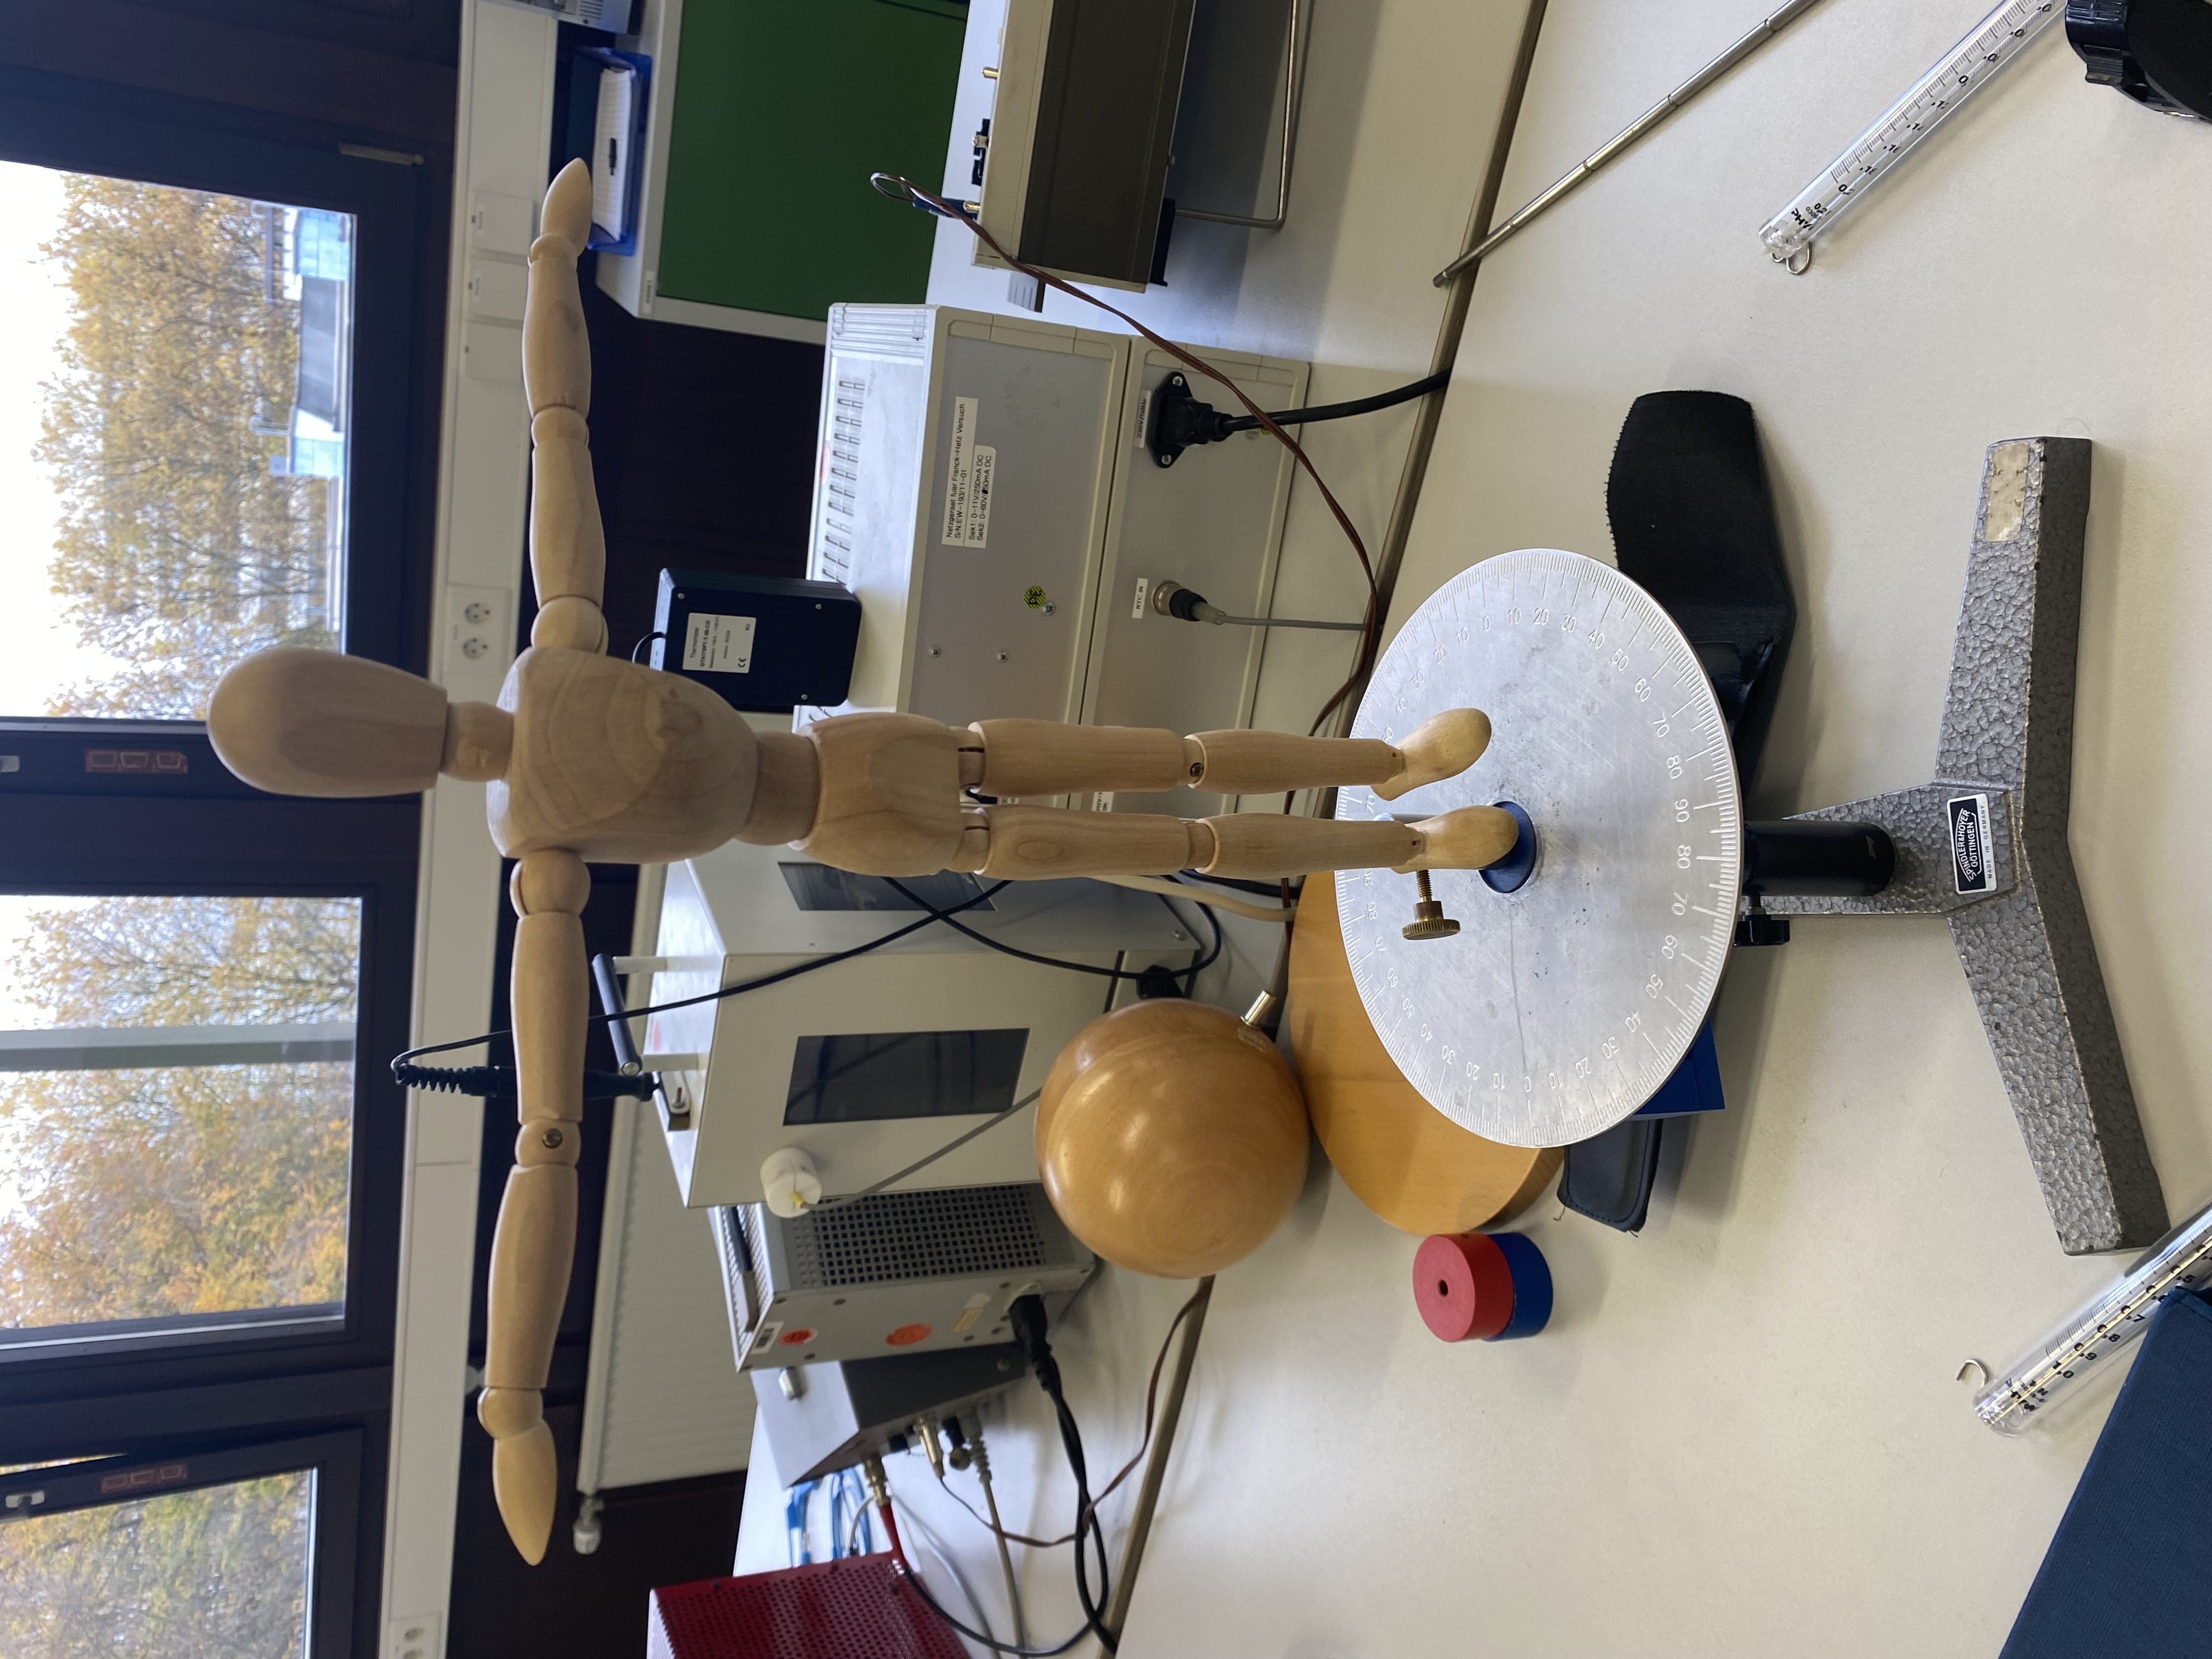
\includegraphics[scale=0.1, angle=270]{Bilder/Stellung1.jpg}
   %     \caption{Stellung 1}
   %    \label{fig:Stellung1}
   %   \end{subfigure}
   %   \begin{subfigure} 
   %     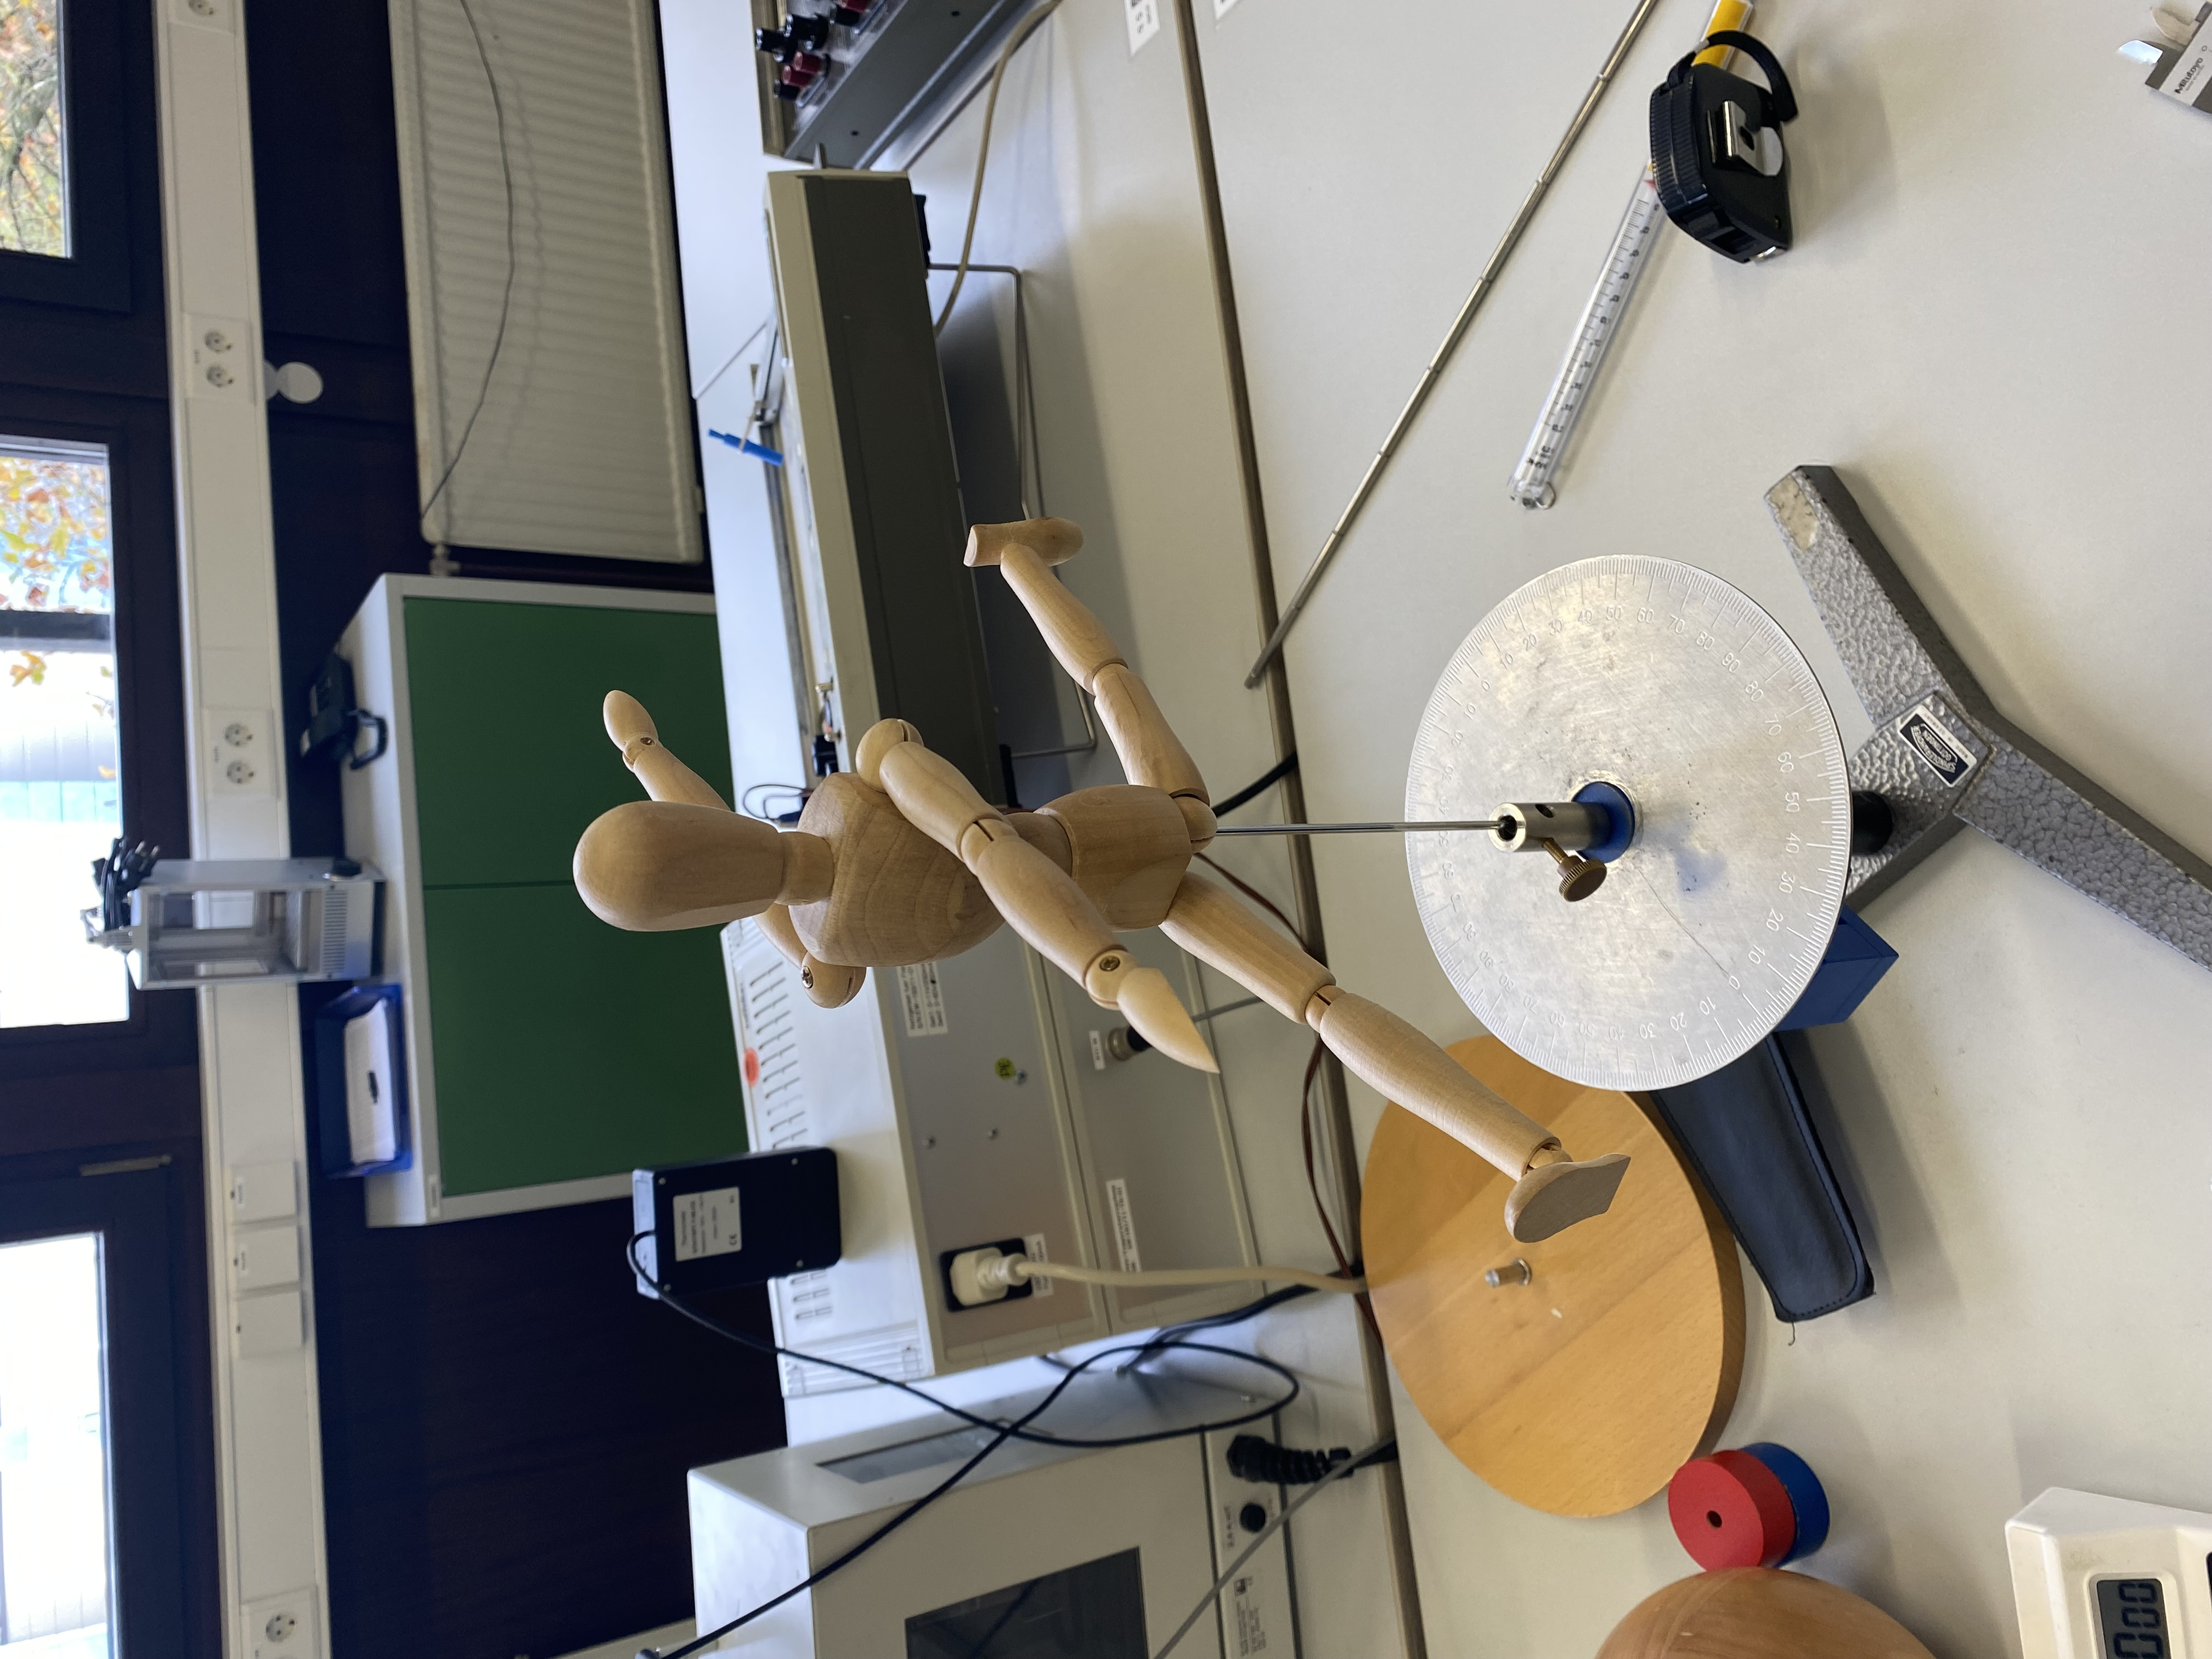
\includegraphics[scale=0.1, angle=270]{Bilder/Stellung2.jpg}
   %     \caption{Stellung 2}
   %     \label{fig:Stellung2}
   %   \end{subfigure}
   % \end{figure}



